% Fixed two-column storyboard:
% <1> Step 1 input video
% <2> Step 2A before optimization
% <3> Step 2B after optimization
% <4-> Step 3 final exported result

\vspace{-0.4cm}
\begin{columns}[T,onlytextwidth]
  % ---------------- LEFT: VISUAL PANEL (changes by step) ----------------
  \begin{column}{0.63\textwidth}
    \begin{outlinecard}[{\only<1>{Input Recording Run}\only<2>{Build Map}\only<3>{ Optimization}\only<4->{Optimized with Tf}}]
      \centering

% STEP 1
      \only<1>{
        \begin{tikzpicture}[x=1cm,y=1cm]
          \draw[draw=NavyBlue!45, line width=0.9pt, rounded corners=1.4pt, fill=white]
            (0.10,0.22) rectangle (7.3,3.9);
          % fixed inner media area (keeps image inside frame)
          \node[inner sep=0pt, anchor=south west] at (0.33,0.50)
          {%
            \IfFileExists{assets/videotrack_fixed_traj_4x.mp4}{%
              \movie[
                width=6.6cm,
                height=3.20cm,
                poster
              ]{%
                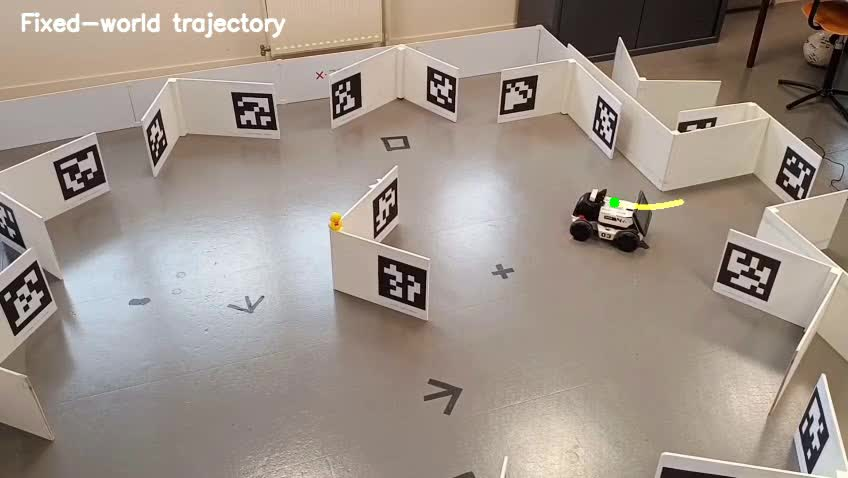
\includegraphics[
                  width=6.6cm,
                  height=3.20cm
                ]{assets/videotrack_fixed_traj_thumb.jpg}%
              }{assets/videotrack_fixed_traj_4x.mp4}%
            }{%
              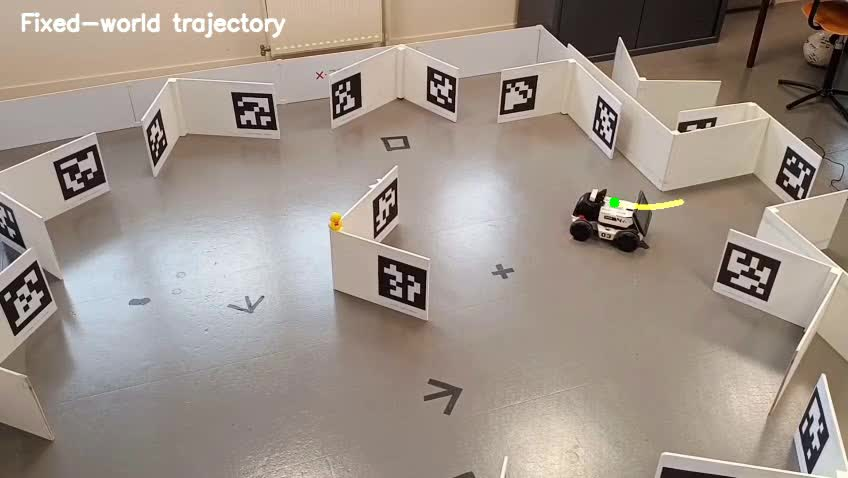
\includegraphics[width=6.6cm,height=3.20cm]{assets/videotrack_fixed_traj_thumb.jpg}%
            }%
          };
          \fill[black, opacity=0.18] (0.33,0.50) rectangle (6.93,3.70);
          \fill[white, opacity=0.92] (3.72,2.10) circle (0.30);
          \fill[NavyBlue] (3.63,1.98) -- (3.63,2.22) -- (3.84,2.10) -- cycle;
        \end{tikzpicture}
      }

      % STEP 2A
      \only<2>{
        \begin{tikzpicture}[x=1cm,y=1cm]
          \node[inner sep=0pt, anchor=south west] at (0.12,0.24)
            {
\includegraphics[width=7cm,height=5cm]{../assets/results/recording_before_no_opt_anchor24.png}};
          \node[anchor=south east, inner sep=0pt] at (8.18,0.6){
            \begin{tikzpicture}[x=1cm,y=1cm]
              \draw[draw=NavyBlue!55, fill=white, rounded corners=0.8pt, line width=0.6pt] (0,0) rectangle (1.35,1.35);
              \draw[AccentBlue, line width=0.9pt] (0.10,1.12) -- (0.34,1.12);
              \node[anchor=west, font=\tiny] at (0.40,1.12) {trajectory};
              \fill[green!70!black] (0.10,0.88) circle (0.025);
              \fill[red!80!black]   (0.25,0.88) circle (0.025);
              \node[anchor=west, font=\tiny] at (0.36,0.88) {start/end};
              \fill[AccentGold] (0.10,0.64) circle (0.025);
              \node[anchor=west, font=\tiny] at (0.20,0.64) {tags};
              \fill[AccentGold] (0.10,0.40) circle (0.033);
              \draw[black, line width=0.4pt] (0.10,0.40) circle (0.033);
              \node[anchor=west, font=\tiny] at (0.20,0.40) {anchor};
              \fill[AccentBlue!45] (0.10,0.16) circle (0.025);
              \node[anchor=west, font=\tiny] at (0.20,0.16) {cloud};
            \end{tikzpicture}
          };
        \end{tikzpicture}
      }

      % STEP 2B
      \only<3>{
        \begin{tikzpicture}[x=1cm,y=1cm]
          \node[inner sep=0pt, anchor=south west] at (0.12,0.2)
            {
\includegraphics[width=7cm,height=5cm]{../assets/results/recording_after_opt_anchor24.png}};
          \node[anchor=south east, inner sep=0pt] at (8.18,0.6){
            \begin{tikzpicture}[x=1cm,y=1cm]
              \draw[draw=NavyBlue!55, fill=white, rounded corners=0.8pt, line width=0.6pt] (0,0) rectangle (1.35,1.12);
              \draw[AccentBlue, line width=0.9pt] (0.10,0.90) -- (0.34,0.90);
              \node[anchor=west, font=\tiny] at (0.40,0.90) {trajectory};
              \fill[green!70!black] (0.10,0.66) circle (0.025);
              \fill[red!80!black]   (0.25,0.66) circle (0.025);
              \node[anchor=west, font=\tiny] at (0.36,0.66) {start/end};
              \fill[AccentGold] (0.10,0.42) circle (0.025);
              \node[anchor=west, font=\tiny] at (0.20,0.42) {tags};
              \fill[AccentGold] (0.10,0.18) circle (0.033);
              \draw[black, line width=0.4pt] (0.10,0.18) circle (0.033);
              \node[anchor=west, font=\tiny] at (0.20,0.18) {anchor};
            \end{tikzpicture}
          };
        \end{tikzpicture}
      }

      % STEP 3
      \only<4->{
        \begin{tikzpicture}[x=1cm,y=1cm]
          \node[inner sep=0pt, anchor=south west] at (0.12,0.24)
            {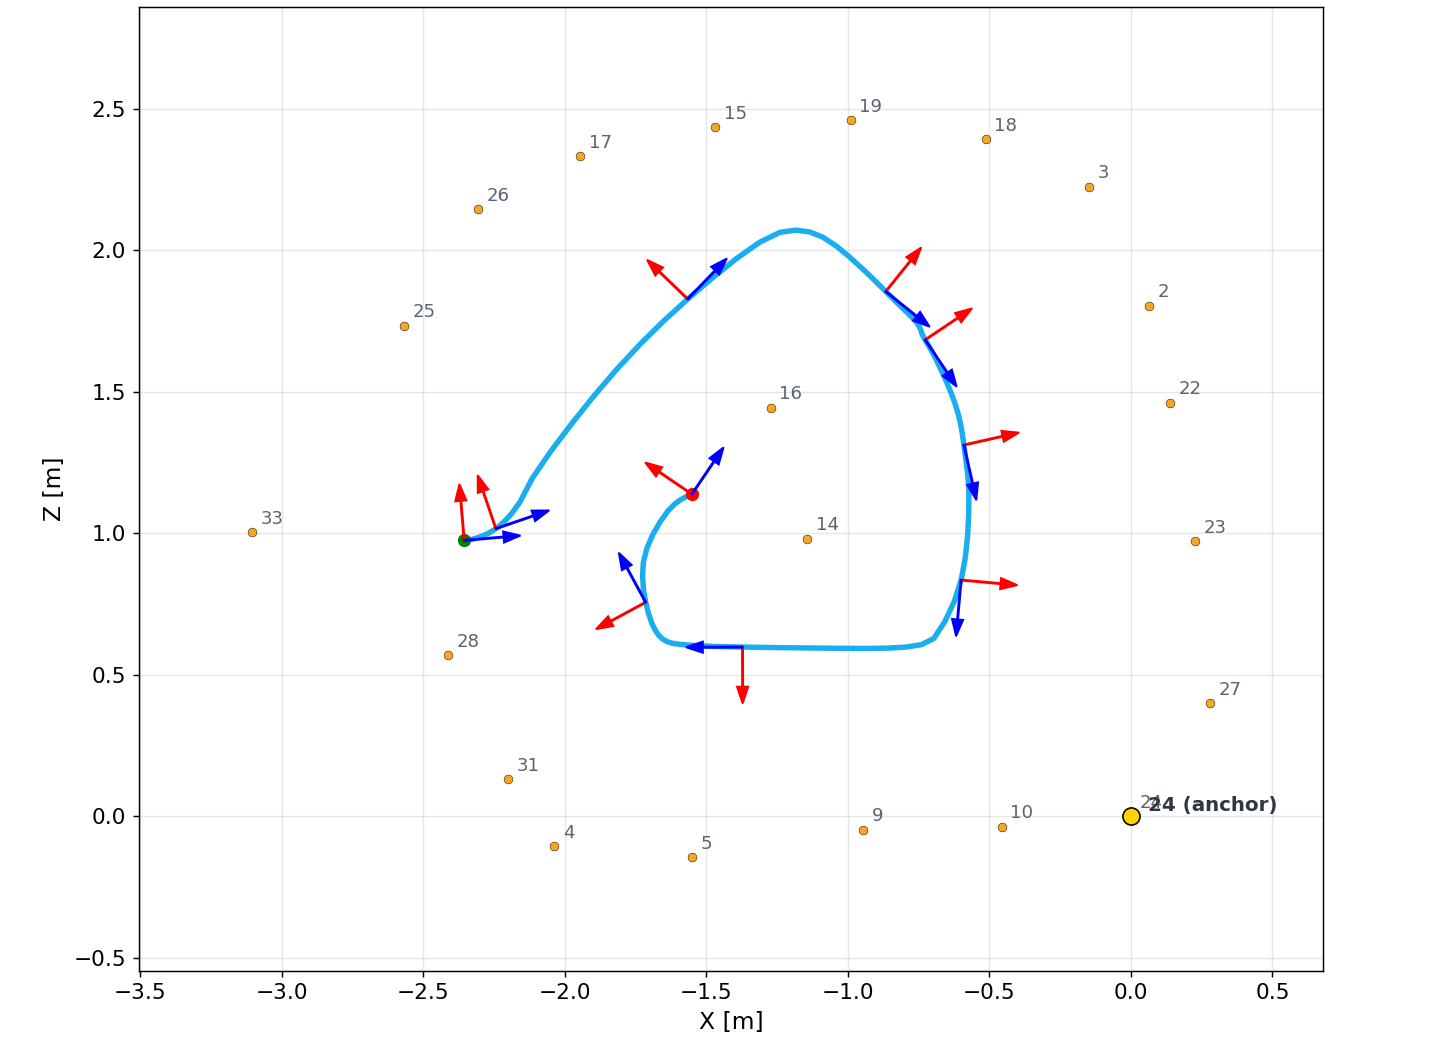
\includegraphics[width=7cm,height=5cm]{../assets/results/recording_final_opt_with_tf_anchor24.png}};
          \node[anchor=south east, inner sep=0pt] at (8.18,0.6){
            \begin{tikzpicture}[x=1cm,y=1cm]
              \draw[draw=NavyBlue!55, fill=white, rounded corners=0.8pt, line width=0.6pt] (0,0) rectangle (1.45,1.35);
              \draw[AccentBlue, line width=0.9pt] (0.10,1.12) -- (0.34,1.12);
              \node[anchor=west, font=\tiny] at (0.40,1.12) {trajectory};
              \fill[green!70!black] (0.10,0.88) circle (0.025);
              \fill[red!80!black]   (0.25,0.88) circle (0.025);
              \node[anchor=west, font=\tiny] at (0.36,0.88) {start/end};
              \fill[AccentGold] (0.10,0.64) circle (0.025);
              \node[anchor=west, font=\tiny] at (0.20,0.64) {tags};
              \fill[AccentGold] (0.10,0.40) circle (0.033);
              \draw[black, line width=0.4pt] (0.10,0.40) circle (0.033);
              \node[anchor=west, font=\tiny] at (0.20,0.40) {anchor};
              \draw[red,  line width=0.7pt, -{Latex[length=1.1mm]}] (0.10,0.16) -- (0.34,0.16);
              \draw[blue, line width=0.7pt, -{Latex[length=1.1mm]}] (0.10,0.16) -- (0.10,0.39);
              \node[anchor=west, font=\tiny] at (0.40,0.16) {axes};
            \end{tikzpicture}
          };
        \end{tikzpicture}
      }
    \end{outlinecard}
  \end{column}

  % ---------------- RIGHT: VERTICAL PIPELINE (always visible) ----------------
  \begin{column}{0.35\textwidth}
    \begin{outlinecard}[Pipeline]
      \centering
      \begin{tikzpicture}[x=1cm,y=1cm,>=Latex]
        \node<1->[draw=NavyBlue!70, fill=white, rounded corners=1.2pt, line width=0.75pt,
          minimum width=3.10cm, minimum height=0.90cm, align=center] (p1) at (1.6,3.05)
          {\scriptsize\textbf{1) Inputs}};
        \node<2->[draw=NavyBlue!70, fill=white, rounded corners=1.2pt, line width=0.75pt,
          minimum width=3.10cm, minimum height=0.90cm, align=center] (p2) at (1.6,1.85)
          {\scriptsize\textbf{2) Build + Optimize}};
        \node<4->[draw=NavyBlue!70, fill=white, rounded corners=1.2pt, line width=0.75pt,
          minimum width=3.10cm, minimum height=0.90cm, align=center] (p3) at (1.6,0.65)
          {\scriptsize\textbf{3) Export}};

        % active step marker
        \fill<1>[AccentGold] ($(p1.north west)+(0.04,-0.04)$) rectangle ($(p1.north west)+(0.15,-0.36)$);
        \fill<2-3>[AccentGold] ($(p2.north west)+(0.04,-0.04)$) rectangle ($(p2.north west)+(0.15,-0.36)$);
        \fill<4->[AccentGold] ($(p3.north west)+(0.04,-0.04)$) rectangle ($(p3.north west)+(0.15,-0.36)$);
        % non-active markers
        \fill<2->[AccentBlue] ($(p1.north west)+(0.04,-0.04)$) rectangle ($(p1.north west)+(0.15,-0.36)$);
        \fill<4->[AccentBlue] ($(p2.north west)+(0.04,-0.04)$) rectangle ($(p2.north west)+(0.15,-0.36)$);

        \draw<2->[NavyBlue!65, line width=0.9pt, -{Latex[length=2.2mm,width=1.6mm]}] (1.6,2.58) -- (1.6,2.30);
        \draw<4->[NavyBlue!65, line width=0.9pt, -{Latex[length=2.2mm,width=1.6mm]}] (1.6,1.38) -- (1.6,1.10);
      \end{tikzpicture}
    \end{outlinecard}

    \vspace{-0.2cm}
    \only<1>{
      \begin{outlinecard}[Step Notes]
        \scriptsize
        \textit{Data acquisition step with rosbag.}
      \end{outlinecard}
    }
    \only<2>{
      \begin{outlinecard}[Equation]
        \scriptsize
        \[
          {}^{\text{world}}\!T_{\mathrm{tag}_i}(t)
          =
          {}^{\text{world}}\!T_{\mathrm{cam}}(t)
          \;{}^{\text{cam}}\!T_{\mathrm{tag}_i}(t)
        \]
      \end{outlinecard}
    }
    \only<3>{
      \begin{outlinecard}[Optimization Equation]
        \scriptsize
        \[
          \min_{\{{}^{w}T_{\mathrm{tag}_i}\}}
          \sum_{(i,j)\in\mathcal{E}}
          \rho\!\left(\|\mathrm{err}_{ij}\|^2\right)
        \]
      \end{outlinecard}
    }
    \only<4->{
      \begin{outlinecard}[Exported Outputs]
        \scriptsize
        \begin{itemize}
          \item \texttt{tag\_map.yaml}
          \item \texttt{trajetoria\_camera.csv}
          \item \texttt{mapa\_tags.csv}
        \end{itemize}
      \end{outlinecard}
    }
  \end{column}
\end{columns}
